\section{Problem Formulation} \label{sec:Problem Formulation}
Our models strongly draws from the previous studies \cite{Xue2016Avi1, Xue2016Avi2}, with modifications directed at reducing computation time, as well as getting better results. Since GPUs enable faster computation on tensors, both the Identification and the Pricing Problem are formulated as tensor-based 3-layered and 2-layered neural networks respectively using the Pytorch library \cite{PTDocs}. Recognizing that NVIDIA GPUs easily pair with Pytorch \cite{PTDocs}, accelerating tensor operations using CUDA and cuDNN \cite{cuDNNPaper, NVIDIA}, we aim to maximize parallel operations and minimize thread synchronization.

\subsection{Identification Problem} \label{sec:Identification Problem}
As discussed in \Cref{sec:Introduction}, the model should learn parameters that caused the change in agents' behavior when a certain set of rewards was applied to locations in the experiment region. Learning those parameters will help us understand how agents behave with a fixed reward distribution, and will enable organizers to redistribute rewards based on that behavior.

Specifically, given datasets $\vect{y_t}$ and $\vect{x_t}$ of agents' visit densities at time $t$, before and after the rewards $\vect{r_t}$ were placed, we want to find weights $\matr{w_1}$ and $\matr{w_2}$ that caused the change from $\vect{x_t}$ to $\vect{y_t}$, considering possible influence from environmental factors $\matr{f}$ and distances between locations $\matr{D}$. Although the original model proposed to learn a single set of weights $\matr{w}$ \cite{Xue2016Avi2}, our proposed model considers two sets of weights $\matr{w_1}$ and $\matr{w_2}$ as it may theoretically result into higher accuracy and lower loss value. Mathematically, the model can be formulated as:
\begin{equation} \label{eqn:iden_problem}
    \begin{aligned}
        & \underset{\matr{w_1}, \matr{w_2}}{\text{minimize}}
        & & Z_I(\matr{w_1}, \matr{w_2}) = \sum_{t} (\omega_t(\vect{y_t} - \matr{P}(\matr{f}, \vect{r_t}; \matr{w_1}, \matr{w_2})\vect{x_t}))^{2}
    \end{aligned}
\end{equation}
where $\omega_t$ is a set of weights (not a learnable parameter) at time $t$ capturing penalties relative to the priority of homogenizing different locations at time $t$. In other words, it highlights if the organizer wishes higher homogeneity at one time unit over another. Elements $p_{u, v}$ of $\matr{P}$ are given as ($\vect{\Theta_i}$ substituted for $\vect{w_i}_v^T$):
\begin{equation} \label{eqn:puv_equation}
p_{u, v} = \frac{\exp(\vect{\Theta_2} \cdot \text{reLU} (\matr{\Theta_1} \cdot [d_{u, v}, \vect{f_{u}}, r_{u}]))}{\sum_{u'} \exp(\vect{\Theta_2} \cdot \text{reLU} (\matr{\Theta_1} \cdot [d_{u', v}, \vect{f_{u'}}, r_{u'}]))} = \frac{\exp(\Gamma_{u, v})}{\sum_{u'}\exp(\Gamma_{u', v})} = \text{softmax}(\Gamma_{u, v})
\end{equation}

To optimize the loss value $Z_I(\matr{w_1}, \matr{w_2})$, the neural network learns the set of weights through multiple epochs of backpropagating the loss using gradient descent. Furthermore, the program preprocesses the dataset to avoid unnecessary sub-epoch iterations and to promote batch operations on tensors.

\subsubsection{Structure of Input Dataset for Identifying Weights} \label{sec:Structure of Input Dataset for Identifying Weights}
\begin{figure}[!htbp]
    \begin{subfigure}{.64\textwidth}
        \centering
        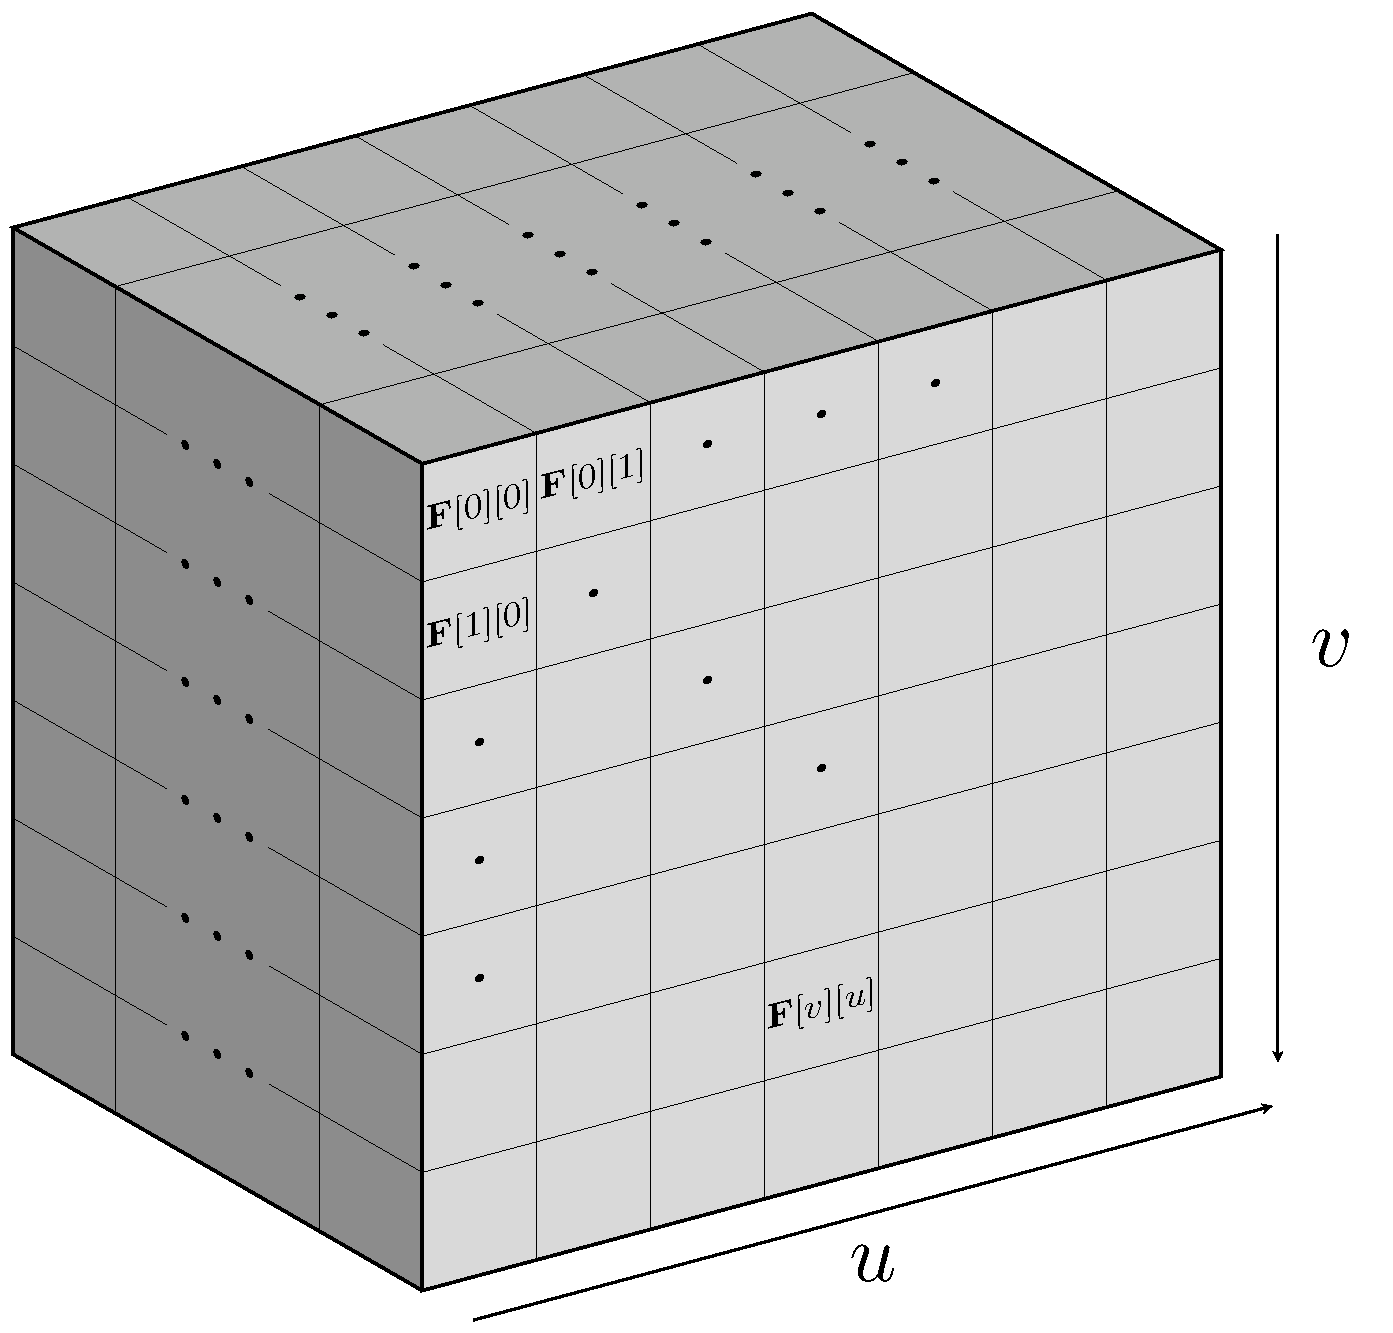
\includegraphics[width=\linewidth]{weights_input_dataset}
        \caption{A Tensor representing the Input Dataset $\tens{F}$}
        \label{fig:A Tensor representing the complete Input Dataset}
    \end{subfigure}
    \begin{subfigure}{.35\textwidth}
        \centering
        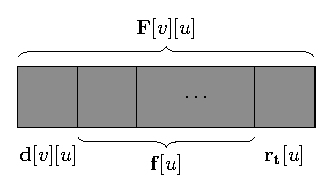
\includegraphics[width=\linewidth]{zoomup_Fuv}
        \caption{Contents of $\tens{F}[v][u]$: This vector (length $n_F$) contains quantified causes for the change in agents' behavior from $\matr{x_t}$ to $\matr{y_t}$}
        \label{fig:Zoomed-in contents of Fvu}
    \end{subfigure}
    \caption{Visual representation of the Input Dataset}
    \label{fig:Visual representation of the Input Dataset}
\end{figure}
Since preprocessing the dataset reduces data operations during model execution, the input dataset, comprising of distance between locations $\matr{D}$, environmental features $\vect{f}$ and given rewards $\vect{r_t}$ (all normalized), is built into a tensor (\Cref{fig:A Tensor representing the complete Input Dataset}) such that operations can be performed on batches of slices $\tens{F}[v]$.

Another advantage of building the dataset as a tensor comes with the Pytorch library, which provides convenient handling and transfer of tensors residing on the Main Memory and GPUs' internal global memory \cite{PTDocs}. \Cref{alg:Constructing the Input Dataset} describes the steps to construct this dataset.
\begin{algorithm}
    \caption{Constructing the Input Dataset} \label{alg:Constructing the Input Dataset}
    \begin{algorithmic}[1]
        \Function{Build-Dataset}{$\matr{D}, \matr{f}, \matr{r_t}$}
        \State $\matr{D} \gets \Call{Normalize}{\matr{D}}$\Comment{$\matr{D}[u][v]$ is the distance between locations $u$ and $v$}
        \State $\vect{f} \gets \Call{Normalize}{\mathbf{f}, axis = 0}$\Comment{$\mathbf{f}[u]$ is a vector of env. features at location $u$}
        \State $\vect{r_t} \gets \Call{Normalize}{\vect{r_t}, axis = 0}$\Comment{$\vect{r_t}[u]$ is the reward at location $u$}
        \For{$v = 1, 2, \dots, J$}
            \For{$u = 1, 2, \dots, J$}
                \State $\tens{F}[v][u] \gets [\matr{D}[v][u], \vect{f}[u], \vect{r_t}[u]]$ \Comment{As depicted in \Cref{fig:Zoomed-in contents of Fvu}}
             \EndFor
        \EndFor
        \State \Return $\matr{F}$
        \EndFunction
    \end{algorithmic}
\end{algorithm}

\subsubsection{Minimizing Loss for the Identification Problem} \label{sec:Minimizing Loss for the Identification Problem}
As shown in \Cref{fig:Neural network designed for the Identification Problem}, the neural network is made of 3 fully connected layers - the input layer, the hidden layer with rectified Linear Units (reLU), and the output layer with softmax$(\cdot)$ function units. The network can also be visualized as a stack of 1-dimensional layers (\Cref{fig:Side view of the network}), with the softmax$(\cdot)$ calculated on the stack's output.
\begin{figure}[!htbp]
    \centering
    \begin{subfigure}{\textwidth}
        \centering
        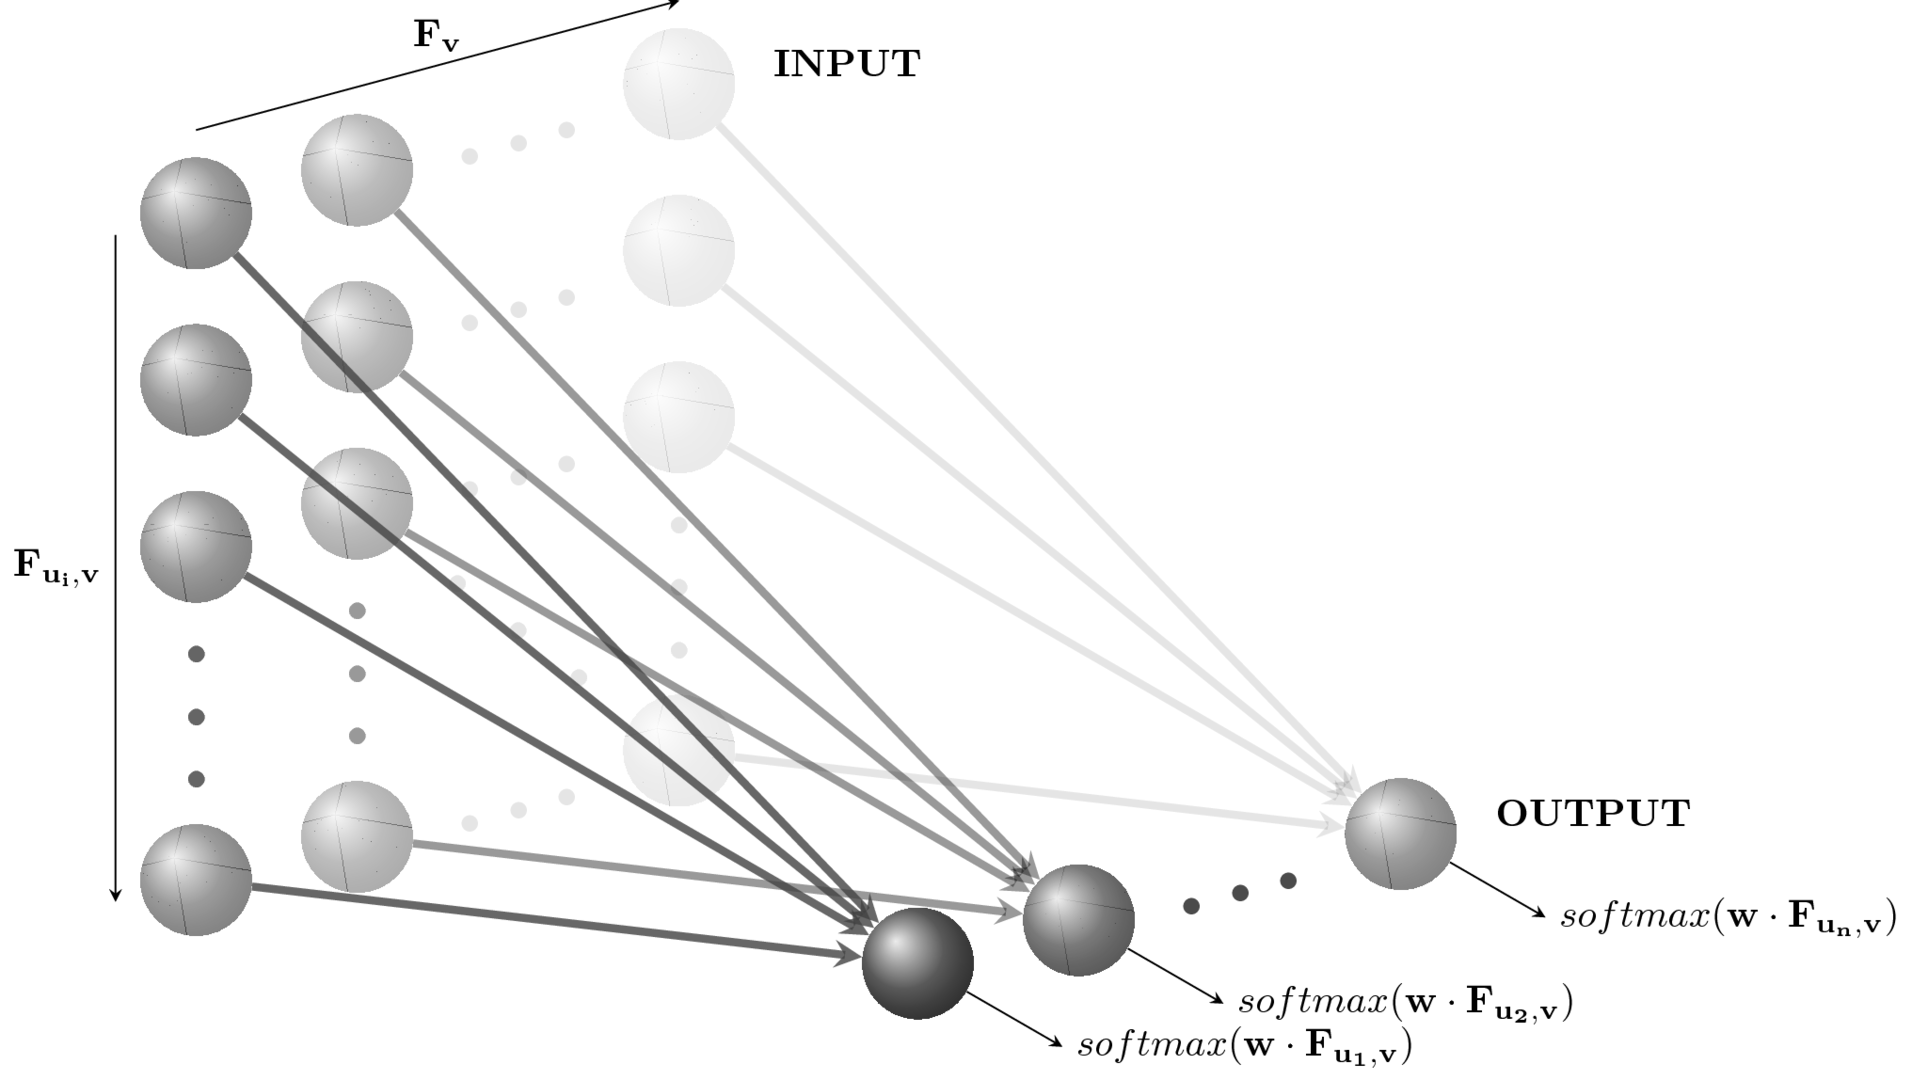
\includegraphics[width=\textwidth]{weights_net}
        \caption{3-dimensional View of the Network Slice, Taking in $\matr{F}[v]$}
        \label{fig:3-dimensional view of the network slice taking in Fv}
    \end{subfigure}
    \begin{subfigure}{.75\textwidth}
        \centering
        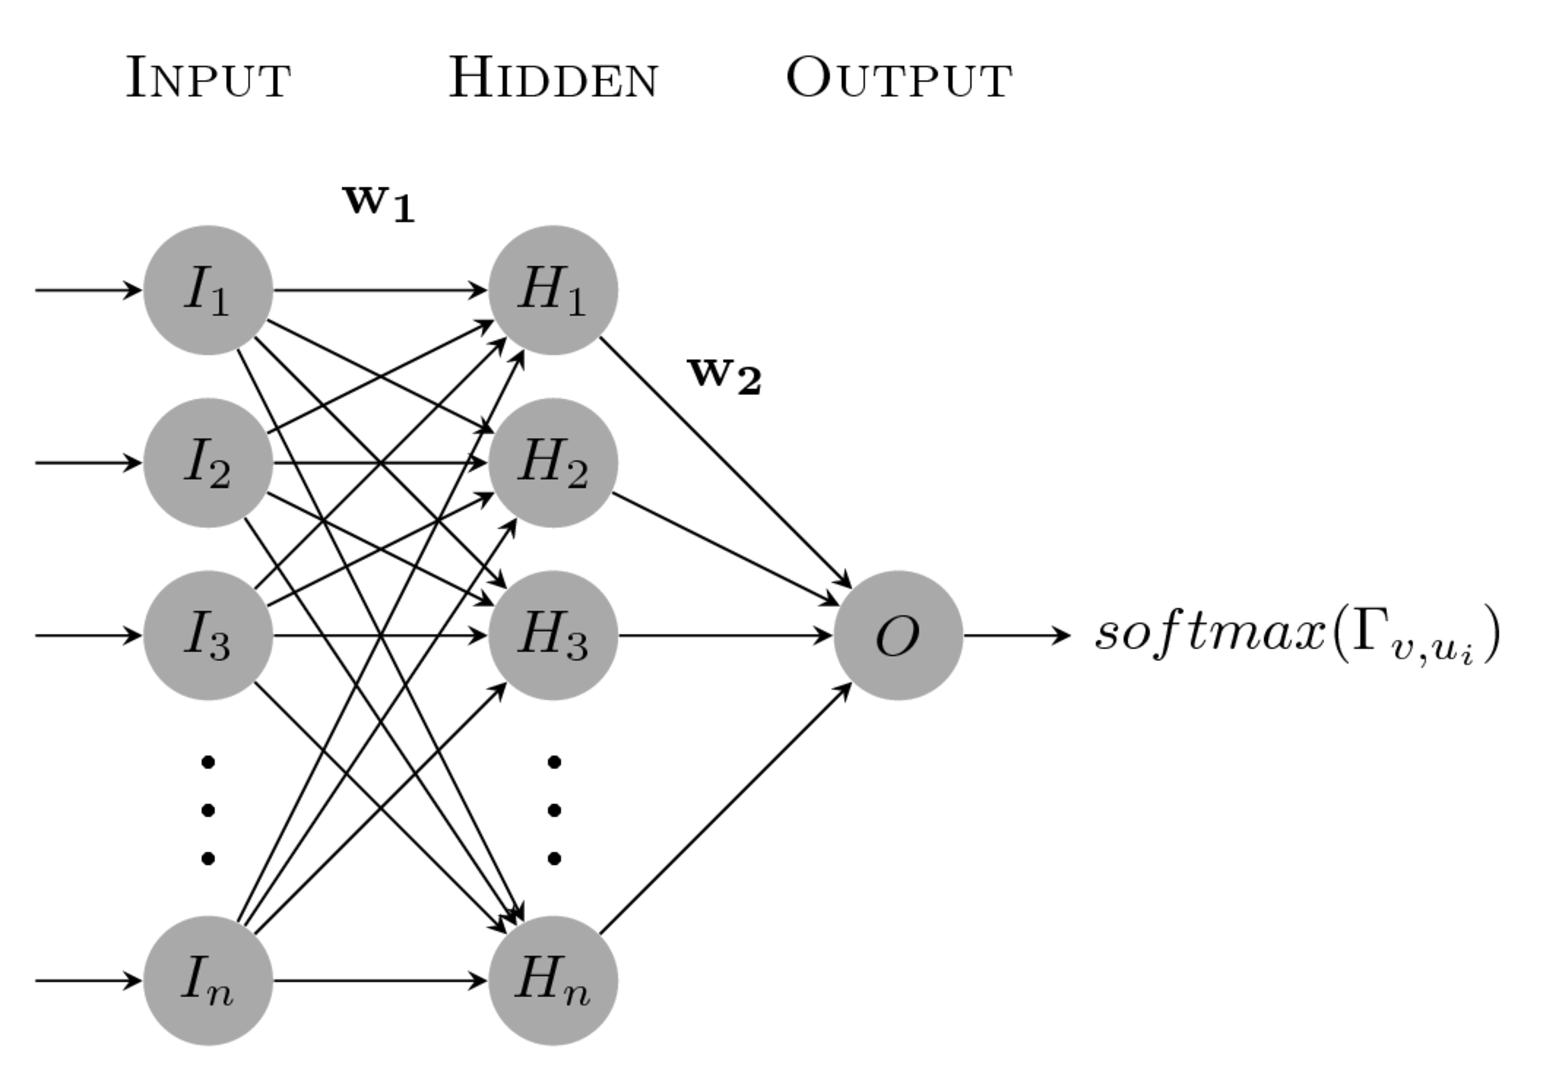
\includegraphics[width=\textwidth]{weights_net_side}
        \caption{Side View of the Network: Output of one such cross-section is $p_{u_i, v}$}
        \label{fig:Side view of the network}
    \end{subfigure}
    \caption{Neural Network Designed for the Identification Problem}
    \label{fig:Neural network designed for the Identification Problem}
\end{figure}

It is important to clarify that the network in \Cref{fig:3-dimensional view of the network slice taking in Fv}, which takes in $\matr{F}[v]$ as shown, is a slice of the original network, which takes in the complete tensor $\matr{F}$ and computes the complete result $\matr{P}^{T}$  per iteration of $t$. In other words, the input and the hidden layers are 3-dimensional, and the output layer is 2-dimensional. Since it is difficult to visualize the complete network on paper, slices of the network are depicted in \Cref{fig:3-dimensional view of the network slice taking in Fv}. \Cref{alg:Algorithm for the Identification Problem} details the steps for learning the parameters $\matr{w_1}$ and $\matr{w_2}$ based on \Cref{eqn:iden_problem,eqn:puv_equation}.

\begin{algorithm}
    \caption{Algorithm for the Identification Problem} \label{alg:Algorithm for the Identification Problem}
    \begin{algorithmic}[1]
        \State $\matr{w_1} \gets \Call{Random}{\;(J,n_F,n_F)\;}$\Comment{$\matr{w_1}$ has dimensions $J \times n_F \times n_F$}
        \State $\matr{w_2} \gets \Call{Random}{\;(J,n_F,1)\;}$\Comment{$\matr{w_2}$ has dimensions $J \times n_F \times 1$}
        \For{$e = 1, 2, \dots, \text{Epochs}$}
            \State $loss \gets 0$
            \For{$t = 1, 2, \dots, T$}
                \State $\matr{F} \gets \Call{Build-Dataset}{\matr{D}, \matr{f}, \matr{r}[t]}$\Comment{Defined in Algorithm \Cref{alg:Constructing the Input Dataset}}
                \State $\matr{H} \gets  \text{reLU}(\Call{Batch-Multiply}{\matr{F}, \matr{w_1}})$
                \State $\matr{O} \gets \text{softmax}(\Call{Batch-Multiply}{\matr{H}, \matr{w_2}})$
                \State $\matr{P} \gets \matr{O}^T$
                \State $loss \gets loss + (\omega(\matr{y}[t] - \matr{P} \cdot \matr{x}[t]))^2$
            \EndFor
            \State $\Call{Gradient-Descent}{loss, \matr{w_1}, \matr{w_2}}$
            \State $\matr{w_1}, \matr{w_2} \gets \Call{Update-Using-Gradients}{\matr{w_1}, \matr{w_2}}$
            \State $\Call{Log-Info}{e, loss}$
        \EndFor
    \end{algorithmic}
\end{algorithm}

\subsection{Pricing Problem} \label{sec:Pricing Problem}
After learning the set of weights $\matr{w_1}$ and $\matr{w_2}$ highlighting the change in agents' behavior to collect observations, the Pricing Problem aims to redistribute rewards to the all locations such that the predicted behavior of agents influenced by the new set of rewards is homogeneous. Thus, given a budget of rewards $\mathcal{R}$, this optimization problem can be expressed as:
\begin{equation} \label{eqn:pricing_problem}
    \begin{aligned}
        & \underset{\vect{r}}{\text{minimize}}
        & & Z_P(\vect{r}) = \frac{1}{n}\lVert \vect{y} - \mean{\vect{y}} \rVert\\
        & \text{subject to}
        & & \vect{y} = \matr{P}(\matr{f}, \vect{r}; \matr{w_1}, \matr{w_2}) \, \vect{x}\\
        &&& \sum_{i} r_i \leq \mathcal{R}\\
        &&& r_i \geq 0
    \end{aligned}
\end{equation}
where elements of $\matr{P}$ are defined as in \Cref{eqn:puv_equation}.

To allocate the rewards $\vect{r}$ optimally, the calculations for the pricing problem are akin to that for the Identification Problem (see \Cref{sec:Identification Problem}). However, since only 1 set of rewards need to be optimized, we use an altered 2-layer (input and output layers) network instead of the 3-layered network used for the Identification Problem. While \Cref{eqn:pricing_problem} looks like a typical Linear Programming problem, only a part of the formulation uses LP to constrain the rewards. We calculate $\matr{P}$ using a 2-layered network that minimizes the loss function $Z_P(\vect{r})$ using gradient descent, and constrain the rewards using linear programming. Fundamental processes are described below, whereas specific implementation details, with code optimizations and more data preprocessing, are described in \Cref{app:Implementation}.

\subsubsection{Input Dataset for Finding Rewards}
Since it is the set of rewards $\vect{r}$ that need to be optimized, they must serve as the ``weights'' of the network (``weights'' here refer to the weighted edges of this network and not to the set of calculated weights $\matr{w_1}$ and $\matr{w_2}$). Therefore, the rewards $\vect{r}$ are no longer fed into the network but are its characteristic. Instead, the calculated weights $\matr{w_1}$ are fed into the network, and are ``weighted'' by the rewards.

The observation density datasets, $\matr{x}$ and $\matr{y}$, are also aggregated for all agents such that they give information in terms of locations $u$ only. This is also why rewards vector $\vect{r}$ does not depend on $t$ - we want a generalized set of rewards for all time $t$ per location $u$. Therefore, the algorithm for constructing $\matr{F}$ (see \Cref{sec:Structure of Input Dataset for Identifying Weights}) is same as \Cref{alg:Constructing the Input Dataset} but with a change - $\vect{r_t}$ replaced by $\vect{r}$.

\subsubsection{Calculating Rewards} \label{sec:Calculating Rewards}
\Cref{alg:Solving the Pricing Problem} for finding $\matr{P}$ is very similar to \Cref{alg:Algorithm for the Identification Problem}'s first few steps but without any epochs of $t$. Also, since the model would predict $\vect{y}$, it does not need labels $\vect{y}$ as a dataset. Although \Cref{alg:Solving the Pricing Problem}'s logic flow may seem arcane, it is straight-forward - as displayed in \Cref{fig:Logic Flow of Algorithm Pricing Problem}.
\begin{figure}[!htbp]
    \centering
    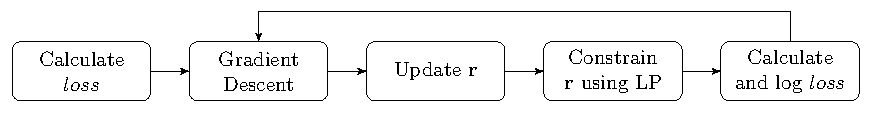
\includegraphics[width=\textwidth]{logic_alg_pricing}
    \caption{Logic Flow of \Cref{alg:Solving the Pricing Problem}}
    \label{fig:Logic Flow of Algorithm Pricing Problem}
\end{figure}
\begin{algorithm}
    \caption{Solving the Pricing Problem} \label{alg:Solving the Pricing Problem}
    \begin{algorithmic}[1]
        \Function{Forward}{$\matr{D}, \matr{f}, \vect{r}, \matr{w_1}, \matr{w_2}, \vect{x}$}
            \State $\matr{F} \gets \Call{Build-Dataset}{\matr{D}, \matr{f}, \vect{r}}$\Comment{Defined in  \Cref{alg:Constructing the Input Dataset}}
            \State $\matr{O}_1 \gets \text{reLU}(\Call{Batch-Multiply}{\matr{F}, \matr{w_1}})$
            \State $\matr{O}_2 \gets \text{softmax}(\Call{Batch-Multiply}{\matr{O}_1, \matr{w_2}})$
            \State $\matr{P} \gets \matr{O}_2^T$
            \State $\vect{y} \gets \matr{P} \cdot \vect{x}$
            \State \Return $\lVert \vect{y} - \mean{\vect{y}} \rVert / J$
        \EndFunction
        \vspace*{-.7\baselineskip}\Statex\hspace*{\dimexpr-\algorithmicindent-2pt\relax}\rule{\textwidth}{0.1pt}%
        \Statex\hspace*{-\algorithmicindent}\textbf{Main Script}%
        \vspace*{-.6\baselineskip}\Statex\hspace*{\dimexpr-\algorithmicindent-2pt\relax}\rule{\textwidth}{0.1pt}% horizontal rule
        \State $\vect{r} \gets \Call{Random}{\;(J)\;}$\Comment{$\vect{r}$ has dimensions $J$}
        \State $loss \gets \Call{Forward}{\matr{D}, \matr{f}, \vect{r}, \matr{w_1}, \matr{w_2}, \vect{x}}$
        \For{$e = 1, 2, \dots, \text{Epochs}$}
            
        \State $\Call{Gradient-Descent}{loss, \vect{r}}$
        \State $\vect{r} \gets \Call{Update-Using-Gradients}{\vect{r}}$
        \State $\vect{r} \gets \Call{LP}{\vect{r}, \mathcal{R}}$\Comment{LP($\cdot$) explained in \Cref{sec:Constraining Rewards}}
        \State $loss \gets \Call{Forward}{\matr{D}, \matr{f}, \vect{r}, \matr{w_1}, \matr{w_2}, \vect{x}}$
        \State $\Call{Log-Best-Rewards}{loss, \vect{r}}$\Comment{Record $\vect{r}$ with the lowest $loss$ yet}
        \EndFor
    \end{algorithmic}
\end{algorithm}

\subsubsection{Constraining Rewards} \label{sec:Constraining Rewards}
After updating the rewards, the program constrains them using LP($\cdot$) such that $\sum_{i}r_i \leq \mathcal{R}$ and $r_i \geq 0$. To do so, the LP($\cdot$) finds another set of rewards $\vect{r'}$ such that the absolute difference between new and old rewards ($\sum_{i}|r'_i - r_i|$) is minimum. The mathematical formulation is given in \Cref{eqn:lp_math_constrain_rewards}, which was implemented using SciPy's Optimize Module \cite{SCPOptimizeDocs}. Since the module supports a standard format for doing linear programming, \Cref{eqn:lp_code_constrain_rewards} is used (see \Cref{app:Implementation}), which is mathematically equivalent to \Cref{eqn:lp_math_constrain_rewards}.
\begin{multicols}{2}
    \begin{equation} \label{eqn:lp_math_constrain_rewards}
        \begin{aligned}\\
            & \underset{\vect{r'}}{\text{minimize}}
            & & \sum_{i}|r'_i - r_i|\\
            & \text{subject to}
            & & \sum_{i}r'_i \leq \mathcal{R}\\
            &&& r_i \geq 0\\ \\
        \end{aligned}
    \end{equation}\break
    \begin{equation} \label{eqn:lp_code_constrain_rewards}
        \begin{aligned}
            & \underset{[\vect{r'}, \vect{u}]}{\text{minimize}}
            & & \sum_{i} u_i\\
            & \text{subject to}
            & & r'_i - r_i \leq u_i\\
            &&& r_i - r'_i \leq u_i\\
            &&& \sum_{i} r'_i \leq \mathcal{R}\\
            &&& r'_i, u_i \geq 0
        \end{aligned}
    \end{equation}
\end{multicols}

We make a tradeoff by constraining rewards using LP instead of Mixed Integer Programming, which the previous study used \cite{Xue2016Avi2}. The tradeoff exists between decreasing the computation time and loosening integer constraints on each reward value. While model-learned integer rewards have worked in real-life testing also \cite{Xue2016Avi2}, we cannot say if allowing non-integer values in rewards would produce better results in real-life, corresponding to the model's prediction. In other words, we can't ensure the predicted rewards' effectiveness in ground testing before \textit{actually} deploying them in the game. Nevertheless, we can estimate how good the predictions can be compared to several baseline indicators. These baseline sets are elaborated in \Cref{sec:Pricing Problem-Optimizing the Original Dataset}.